The following Sections describe the methods used in the course of this thesis.

\subsection{Datasets}\label{subsec:datasets}

Two different datasets were used to train the models.

\subsubsection{CelebA}

\begin{wrapfigure}[11]{r}{0.3\textwidth}
    \begin{center}
        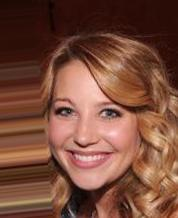
\includegraphics[width=0.28\textwidth]{images/celeba_sample_63.jpg}
    \end{center}
    \caption[CelebA dataset sample image]{A sample image from the CelebA dataset.}
    \label{fig:celeba_sample}
\end{wrapfigure}

The \textit{CelebA} dataset~\citep{liu2015faceattributes} consists of 202,599 RGB images of size 178 x 218 pixels representing celebrities, as well as 40 binary attributes.
The images belong to 10.177 unique identities\footnote{The identities are not revealed.} as well as five \say{landmark annotations}.
They are aligned and cropped resulting in images of same size always showing only one face (see Figure~\ref{fig:celeba_sample} for an example).
The landmark annotations give the positions of facial attributes in the image, specifically of the left and right eye, the nose, and the left and right corner of the mouth.
The binary attributes indicate if the image has certain attributes, for example if the person wears eyeglasses, has black hair, is smiling, etc\footnote{See \href{https://www.kaggle.com/jessicali9530/celeba-dataset\#list\_attr\_celeba.csv}{https://www.kaggle.com/jessicali9530/celeba-dataset\#list\_attr\_celeba.csv} for a complete list of the attributes, login required. Last access: 12/02/2020.}.

\subsubsection{ImageNet}\label{ssec:imagenet}

ImageNet\footnote{\href{http://image-net.org/}{http://image-net.org/}, last access: 12/02/2020.} is a large-scale \say{image database organized according to the WordNet hierarchy}~\citep{imagenet_cvpr09} consisting of over 14 million images as of February 2020.
Accordingly to WordNet\footnote{See \href{https://wordnet.princeton.edu/}{https://wordnet.princeton.edu/}, last access: 12/02/2020.}, on different levels of granularity, the images are subdivided into groups called \say{synsets}~\citep{imagenet_cvpr09}.
For example, the group \textit{woman, adult female} is subordinated to \textit{person, individual, someone, somebody, mortal, soul} and is further subdivided into groups like \textit{old woman} or \textit{lady} \footnote{ImageNet 2011 Fall Release, \href{http://image-net.org/explore}{http://image-net.org/explore}, last access: 12/02/2020.}

A smaller version of ImageNet, commonly called \textit{ILSVRC2012} has been used for \ac{ILSVRC2017}~\citep{ILSVRC15}, consisting of approximately 1,3 million images from 1000 different classes, that were selected, such that \say{there is no overlap between synsets: for any synsets $i$ and $j$, $i$ is not an ancestor of $j$ in the ImageNet hierarchy}~\citep{imagenet_cvpr09}.

This curated version is commonly used as a baseline (\textbf{refs}).

\subsubsection{MNIST}\label{subsubsec:mnist}

\begin{wrapfigure}[10]{r}{0.2\textwidth}
    \begin{center}
        
\includegraphics[width=0.18\textwidth]{images/mnist_sample.png}
    \end{center}
    \caption[MNIST dataset sample image]{A sample image from the MNIST dataset.}
    \label{fig:mnist_sample}
\end{wrapfigure}

MNIST\footnote{\href{http://yann.lecun.com/exdb/mnist/}{http://yann.lecun.com/exdb/mnist/}, last access: 23/04/2020}~\citep{lecun1998gradient} is a widely-used dataset of hand-written digits.
The data is subdivided into a training set of 60.000 images and a test set containing 10.000 images.
The digits are \say{size-normalized and centered}.
The samples are grayscale-images of size $28\times 28$pixels.

\subsubsection{Morpho-MNIST}\label{subsubsec:morphomnist}

Morpho-MNIST~\citep{castro2019morpho} is an extension of the MNIST dataset that addresses the question: \say{[T]o what extent has my model learned to represent specific factors of
variation in the data?} ~\citep{castro2019morpho}.
To address this questions, Morpho-MNIST provides the following (continuous) labels of morphological attributes of the MNIST samples: stroke length, stroke thickness, slant, width, and height.

Besides providing additional labels of low-level MNIST attributes, Morpho-MNIST provides a toolbox to measure (i.e. calculate the morphological labels) and perturb MNIST images.
The perturbation toolbox allows it to thin, thicken, swell, and to add fractures to an image.
Morpho-MNIST also provides pre-computed datasets that were built using the perturbation toolbox.

\subsection{Visual Features Variational Autoencoders}\label{subsec:visual-features-variational-autoencoders}
Different questions were asked investigate whether \acp{VAE} are a biologically plausible model of the Visual Cortex.

One essential prerequisite is the emergence of Gabor wavelets (\textbf{Ref}).
As discussed in Section~\ref{subsec:visual_features_in_neural_networks}, Gabor wavelets do emerge in deep convolutional networks, trained on image classification~\citep{krizhevsky2012imagenet} (\textbf{Ref: at least one more paper }), specifically on the ImageNet dataset (\textbf{ref}).\par
The following approaches were taken to see if Gabor wavelets do naturally emerge in \acp{VAE} (\textbf{explain \say{naturally}}).\par
First, the convolutional kernels in a \ac{VAE} that was sucessfully trained on the CelebA (\textbf{ref}) dataset in terms of image reconstruction were examined in terms of emergence of Gabor wavelets (\textbf{explain network architecture}).
Subsequently, the size of the convolutional kernels in the first layer was increased to size 11x11 \footnote{This is the same kernel size of the first layers used in~\citet{krizhevsky2012imagenet}.} as they were too small to successfully represent any Gabor wavelets~\citep{han2019variational}.
Since still no Gabor wavelets emerged (see Section~\ref{subsec:results_visual_features_in_variational_autoencoders}), the question was raised whether this was because of the different network architectures of AlexNet and the \say{CelebA VAE}, or the dataset, or both.

\begin{figure}
    \centering
    \begin{subfigure}{.5\textwidth}
        \centering
        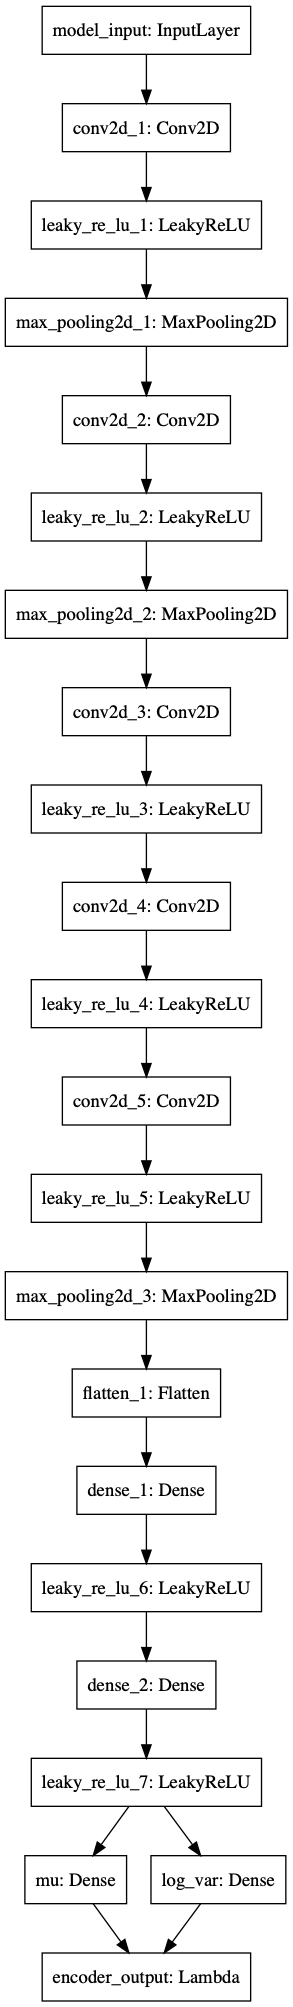
\includegraphics[width=\textwidth,height=.9\textheight,keepaspectratio]{alexnet-vae/encoder.png}
        \caption{Encoder}
    \end{subfigure}%
    \begin{subfigure}{.5\textwidth}
        \centering
        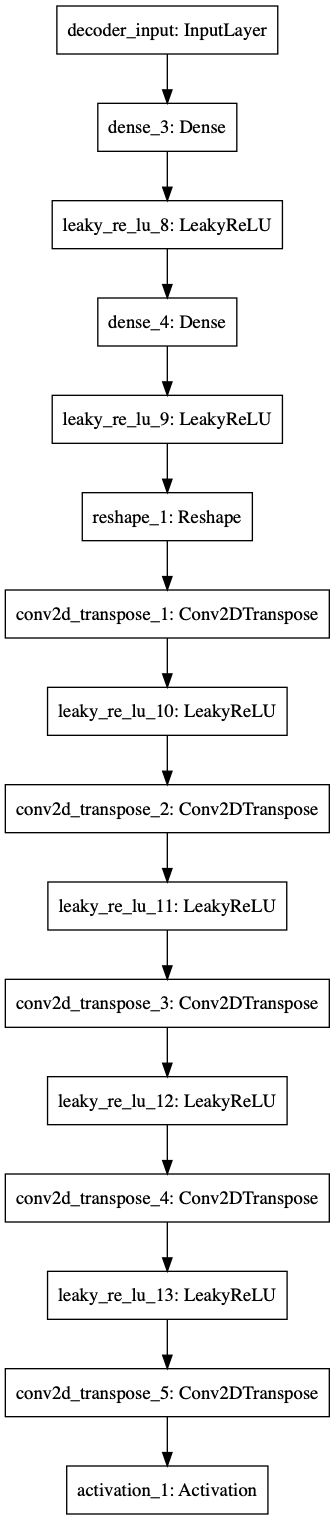
\includegraphics[width=\textwidth,height=.9\textheight,keepaspectratio]{alexnet-vae/decoder.png}
        \caption{Decoder}
    \end{subfigure}
    \caption{AlexNet-VAE Network}
    \label{fig:alexnet-vae-encoder}
\end{figure}

To further localize the so-far cause for the non-existence of Gabor wavelets, an \say{AlexNet-like-VAE} (subsequently called AlexNet-VAE, see Figure~\ref{fig:alexnet-vae-encoder}) was trained on ImageNet.
This \ac{VAE} consists of an encoder part that closely resembles AlexNet.
The output-layer, however, was changed in terms of size and activation function.
First of all, the output size was allowed to be dynamical to allow different embedding sizes, i.e. differently sized multivariate Gaussians.
Also, the activation function was changed from Softmax (\textbf{ref}) to \ac{LeakyReLU} (\textbf{ref}).
Furthermore, all other activations were also changed to \ac{LeakyReLU} due to its advantages over \ac{ReLU} (\textbf{which ones? explain}).
The encoder is was followed by the reparametrization layer and, subsequently, the decoder part which basically consists of the inverse AlexNet structure.\par

\begin{figure}
    \centering
    \begin{center}
        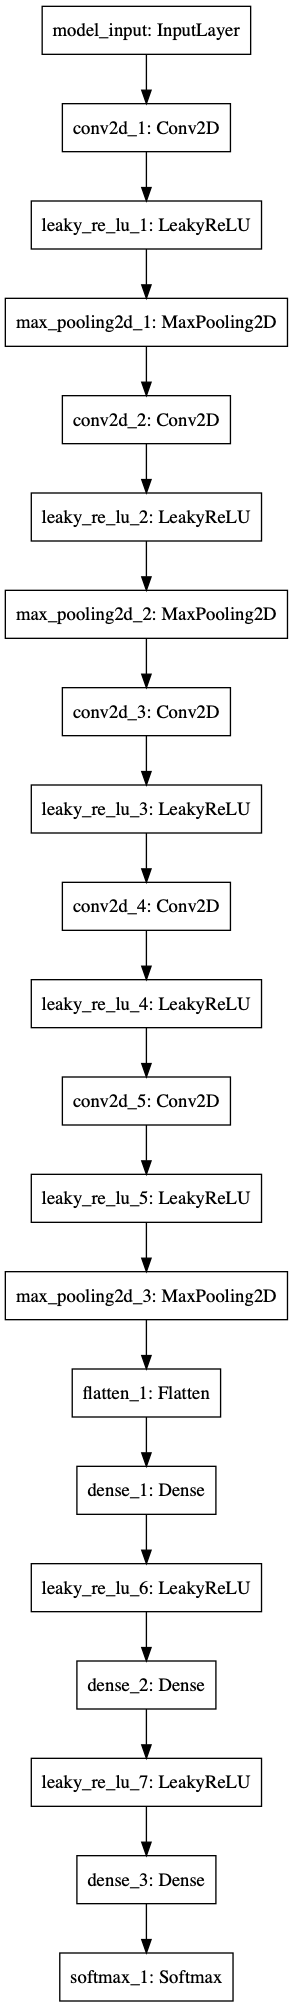
\includegraphics[height=0.9\textheight]{alexnet/model.png}
    \end{center}
    \caption[AlexNet Network]{AlexNet-inspired Image Classification Network}
    \label{fig:alexnet}
\end{figure}

To cross-check the results of the AlexNet-VAE, only the encoder part was trained on ImageNet and image classification, using the Softmax activation in the last layer but keeping the \ac{LeakyReLU} activations in all other layers (see Figure~\ref{fig:alexnet}).

As it turned out that also in the AlexNet-VAE no Gabor wavelets emerged (see Section~\ref{subsec:results_visual_features_in_variational_autoencoders}), the image classification AlexNet-like network was used as an encoder with frozen weights and only the decoder part was trained to see if using a network trained on image classification has certain disadvantages when being used as a decoder in a \ac{VAE} compared to a decoder trained from scratch.

\subsection{Activity Correlation in \acp{VAE}}\label{subsec:activity-correlation-in-vaes}

It is known from the visual cortex that the activity following a visual stimulus is propagated forwards and backwards (\textbf{ref}).
Therefore, the question was asked whether \acp{VAE} do something similar, i.e.\ if the activity in the encoder is similar to the activity in the encoder.
Here, the activity $a(o_x(\mathcal{K}_{l,i}))$ is defined as the sum over the values of a certain feature map $o_x(\mathcal{K}_{l,i})$ , i.e.\ the result of the $i$-th convolution $\mathcal{K}_{l,i}$ in the $l$-th layer
\begin{align}
    a(o_x(\mathcal{K}_{l,i})) = \sum_n \sum_m o_x(\mathcal{K}_{l,i})
\end{align}
with $n$ and $m$ indicating the rows and, respectively, the columns of the feature map $o_x(\mathcal{K}_{l,i})$.

In order to compare the activities, each layer in the encoder is matched to its counterpart in the decoder.
This is possible because encoder and decoder are structured completely symmetrically: Each convolution in the encoder corresponds to a deconvolution in the decoder.

However, as the order of feature maps in one layer is determined by chance, it is not reasonable to expect that the $i$-th feature map in the $l$-th encoder-layer has the same semantic significance as the $i$-th feature map in the counterpart in the decoder.
Therefore, an order is induced by ordering the feature maps by their activity $a(\cdot)$ given a certain stimulus $x$.
Given this order, the Pearson correlation coefficient~\citep{freedman2007statistics} is calculated by
\begin{align}
    \rho_{X, Y} = \frac{E[(X- \mu_X)(Y- \mu_Y)]}{\sigma_X \sigma_Y}
\end{align}
where $X$ and $Y$ are the flattened and under consideration of the order matched feature maps, $\mu_X = E[X]$ is the expectation, and $\sigma_X$ the standard deviation.
